%!TEX root = thesis.tex
\chapter{Implementation and experiments}
This Chapter firstly describes how the testing platform is set up to assess the performance of different types of compressed CityJSON.
Then, I explain the way in which the operations defined in Section~\ref{methtestingplatform} are performed on the testing platform, and subsequently give information on the performance benchmark,.
After that comes the implementation of the compression types of Section~\ref{sec:compressionimplementation} and a description of the datasets on which these are tested.
Lastly I present the results of experiments that do not directly belong in Chapter~\ref{ch:bmresults} but analyse the lossiness of compression types, helped with making implementation choices, or are relevant in other ways.
Tools that are used for the implementation are briefly described in Appendix~\ref{ch:tools}.


\label{ch:impl}
\section{Flask server}


The Flask server is the base of the testing platform introduced in Chapter~\ref{ch:meth}.
Flask is a lightweight Python web framework with which web applications can be built \citep{Flask2020}.
It enables combined use of Python and JavaScript, where the former handles the transmission of data (from datasets that are stored on the server) to the client, while the latter handles the processes that are performed in the client, such as the visualisation.
In this way, CityJSON files (and compressed variants) can be used on the web, with operations performed on it on either the server or in the client.

The testing platform is set up in \ac{rest}ful \citep{Fielding2000} style---with a clear separation between the client and the server, and having stateless communication between these two, which means that every request to the server needs to contain all necessary information to fulfill the request as the server does not remember previous interactions with the client.
In Flask, routes (in the form of URLs) are defined in the server's code and coupled with a function that is executed when the specific route is visited, \ie\ the client makes a request to the server.
For the testing platform I have created routes and corresponding functions that enable to perform the operations laid out in Table~\ref{tab:operationnames}.
When such a function is finished, it returns an html template that is rendered in the client, a dataset (that is prepared on the server if applicable), and variables with information on the current operation so that the client knows how the process the data.

There are two different server implementations: one with the compression of datasets beforehand, and one with compression on the fly.
As for the first one, all datasets are compressed by every compression types and these files can be requested from the server.
Compressed files can not be manipulated before decompressing them (however, see Section~\ref{querycompressed}).
Since the presumed advantage of using compressed files on the web is the mitigation of the data transfer time from server to client, decompressing and performing an operation on a dataset on the server is unwanted because it would diminish this potential speed gain.
Therefore, the server transmits the full compressed dataset to the client, which will proceed to decompress it and execute the specified operation.
For a fair comparison, operations on original CityJSON data are also performed in the client, despite the possibility to process them before transmission.

With the second implementation, an original CityJSON dataset is always loaded by the server after a request has been made.
The specified operation is then performed on it (except for visualisation, which can only be done in the client), and if necessary the processed data is then compressed before transmission.
This means that it is possible to only transmit a selection of city objects rather than having to send them all.
But because now the compression time is of importance for the time that is lapsed finishing an operation, this could hamper the performance of compression types, especially when they take long.

In Figure~\ref{fig:testingplatform}, an overview of the server implementation used in this thesis is shown.
It is further explained in Section~\ref{sec:testingplatformoverview}.


\begin{figure}[h!]
    \hspace*{-1.8cm}  
    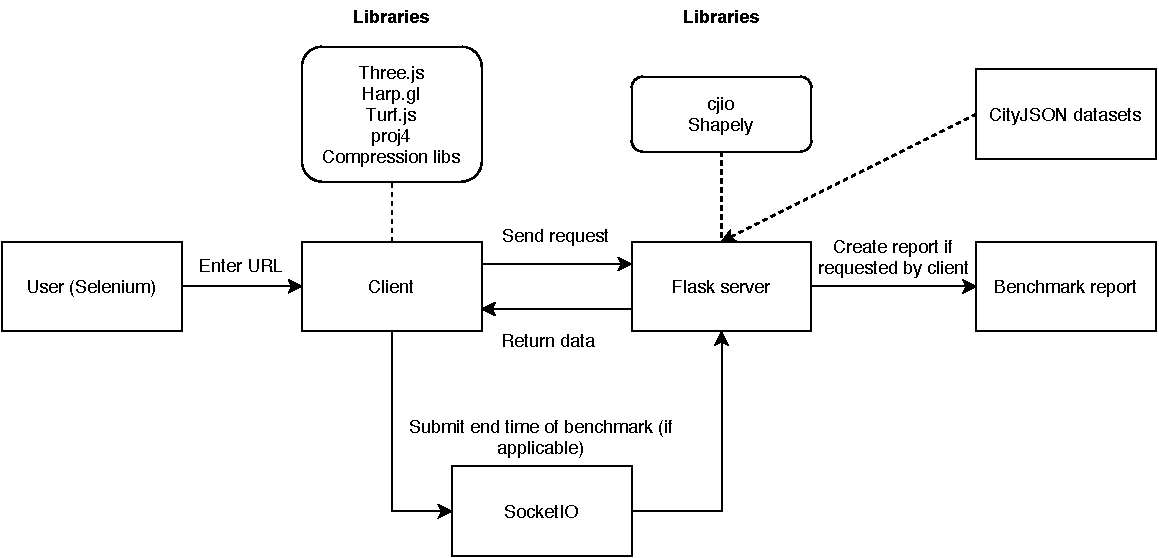
\includegraphics[scale=0.95]{figs/implementation/Testing platform.pdf}
    \caption{Diagram showing an overview of the structure of the testing platform.}
    \label{fig:testingplatform}
\end{figure}



\subsection{Three.js}
\label{sec:threejsmesh}

Three.js \citep{Three.js2020} is used for the visualisation of the datasets.

It is a higher level 3D library for JavaScript that helps visualising 3D geometries by providing functions that ultimately render graphics through the lower level WebGL.
% https://github.com/mrdoob/three.js/
WebGL has the ability to visualise 3D graphics in the browser using hardware acceleration, allowing for greater performance compared to using the CPU only \citep{WebGL2011}.
In its coordinate sytem, geometries are being centered around the origin and their coordinates normalised, such that all fall within the range \texttt{[-1, 1]}.
% not clear whether or not the coordinate system is left- or right-handed in WebGL, might be both or neither. Long discussion on stackoverflow about this. Therefore I don't specify this as I don't want to dive deep into that.
Objects can thus have negative coordinates and they are not georeferenced in Three.js \citep{Three.js2020}.

The CityJSON viewer \citep{Boersma2019} contains code that parses CityJSON geometries into a Three.js mesh.
Using this the CityObjects can be visualised. 
Part of this code is used in the testing platform, to be used for data that has its geometries stored in CityJSON's native manner rather than as a Draco blob.

A Three.js mesh is always formed only of triangles and can contain one material \citep{Three.js2020a}.
Within a mesh object, the geometry can be stored in two manners.
It can be stored in the mesh similarly to OBJ and CityJSON (see Section~\ref{sec:cityjsonexplained}): as a combination of three-dimensional vectors as coordinates and triangular faces with index references to the vectors.
Such an object is named a \texttt{Geometry} in the library and this is what the CityJSON viewer parses geometries of datasets into.
The alternative is a \texttt{BufferGeometry} object \citep{Three.js2020b}, which is less user-friendly but processed more efficiently.
It simply contains an array of coordinates as floats, which would represent a matrix.
This is one similarly for the faces.
The Draco decoder for JavaScript decodes a Draco blob into a BufferGeometry.
This difference can have an impact on the benchmarking results.







\subsection{cjio}
cjio \citep{cjio} stands for CityJSON input/output.
It is a Python command-line interface that has several functions that can be used to work with CityJSON files.
It can be used to help preparing CityJSON datasets for the testing part, but more importantly, it can facilitate the querying and analysis of the datasets by integrating it with Flask and possibly Python libraries such as Shapely \citep{cjio}.
I chose to host files on the server and process queries with cjio and other tools, but another option is to use a \ac{dbms} such as 3DCityDB \citep{TUM2020}.


\subsection{Draco}
\label{sec:dracoimplementation}
As explained in Section~\ref{rwdraco}, Google's Draco library is an open-source library to compress and decompress 3D geometric meshes for the purpose of improved storage and transmission efficiency.
It is used for the compression of the geometrical part of CityJSON's file structure\citep{draco}.

The Draco library includes an encoder and decoder for JavaScript, which can conveniently be used in the testing platform.
Three.js has a function which decodes Draco using the previously mentioned decoder and loads it as a mesh that can subsequently be visualised.
However, as opposed to Draco's C++ decoder, the one in JavaScript lacks the functionality for separating sub-objects (as features or CityObjects are called in Draco)---it would create one large mesh out of the Draco geometry.
This makes it impossible to query objects which is necessary for several of the operations (see Section~\ref{sec:operations}) in this thesis.

Therefore, I have altered the inner workings of the JavaScript decoder.
I have added a part that is supposed to enable the passing of one or more object IDs, making it only return these specified objects as a mesh.
This is only possible after the Draco blob has been fully decoded, adding time to the process.
% https://github.com/google/draco/issues/401
This is done by iterating over all faces of the decoded Draco geometry, querying the sub-object ID from its first vertex from a metadata querying function of Draco, and checking if it equals one of the IDs that had been previously passed to the decoder.

Additionally, the three.js function does not allow passing a Draco \ac{blob} directly but requires a link instead.
This link is subsequently downloaded into a BytesArray after which it is decoded. 
For this reason, Draco files are downloaded separately by visiting a Flask route.
The Draco parts are taken out of the compressed CityJSON files in order to not affect the transmission speed and thus the benchmarking results.

The encoder, which is used after editing a file, can be used unaltered.
However, it is not possible to choose a compression level between 0 and 10 like the C++ encoder can, but instead a choice can only be made between using Edgebreaker (Subsection~\ref{sec:theoryedgebreaker}) and the sequential connectivity encoding method (Subsection~\ref{sec:seqconnectivity}).
% which one do I use and why?
% code taken from tutorial: https://github.com/google/draco/

\subsection{Testing platform overview}
\label{sec:testingplatformoverview}
The diagram of Figure~\ref{fig:testingplatform} shows an overview of the testing platform.
The user (who is simulated by Selenium for the benchmarking---see Section~\ref{implselenium}) sends a request through the client to the Flask server.
Subsequently the server processes the request and data if needed (if compression is done on the fly), and starts a timer for the benchmarking.
It then returns the requested data (the full CityJSON file or a compressed variant in the case of compression in advance) and information on the requested operation to the client.
The client parses the data (decompressing it if necessary) and finishes the operation.
Both the client and server are supported by several libraries.
Once the operation is finished, it will emit a message with the end time of the benchmark to SocketIO \citep{Socket.io2020}, which allows communication between JavaScript and Python.
Socket.io in turn sends the message to the Flask server.
The latter calculates the time that has lapsed and stores this, and a report of the benchmark is created when requested by the user.



\section{Operations}
\label{sec:operations}

The way in which operations are implemented influences the time benchmarking results.
Additionally, they can be different for varying data types, and understanding what is happening under the hood helps with reasoning why the results of compression types turned out as they did.

In every case, once the client makes a request to the server, the server stores the starting time of the process.
It then processes uncompressed CityJSON (and compresses) if needed and stores the result as a file.
Flask will then render a \ac{html}, while submitting information to the client about the process---the name of the requested dataset, the compression type, and the operation name.
The information is used to enable the client to parse the correct URL with which the needed file can be downloaded.



\subsection{Visualisation}
As the file that needs to be visualised is downloaded, it is decoded as described in Section~\ref{sec:compressiondecompression} if necessary.
If it contains original CityJSON geometry objects, these are converted into a three.js mesh using code based on the CityJSON viewer.
Otherwise, the JavaScript Draco decoder is used to convert the Draco geometry to a three.js mesh.
In that case also the object IDs to which every vertex belongs has to be queried using \texttt{MetadataQuerier()} of the Draco decoder.
This is necessary because the Draco decoder creates one large mesh out of all objects, making it impossible to link attributes to separate objects.
When visualising a 3D city model it is important that this can be done, and it makes the comparison to the visualisation of Geometry Objects fair.

When this is finished, the three.js mesh is added to the harp.gl map and visualised.
The client then returns the current time to the server, which will calculate the time that has lapsed and add it to the benchmarking report.


\subsection{Querying}
\subsubsection{Querying one object}
\label{sec:queryone}
The first object of the dataset is queried on its ID.
With compression on the fly this is done on the server, otherwise in the client.
The queried city object is taken by accessing the value of the ID as key in the \texttt{"CityObjects"} member of the CityJSON object.
It is placed in a new CityJSON object, and its geometry is then processed by cjio's "subset.process\_geometry" function, retaining only the vertices that belong to the object and updating the vertex indices in the geometry object to start with 0.
The bounding box is updated, and the CityJSON object is then stored in a file and can be downloaded by the client.
As the download is completed, the client will submit the end time to Flask.
Since cjio does not exist for JavaScript I have translated the "subset.process\_geometry" function to it, in case the querying is done in the client.

With Draco geometries, the difference is that the vertices corresponding to the object ID need to be found with "\texttt{MetadataQuerier()} of the Draco decoder.
As explained in Section~\ref{sec:dracoimplementation} however this does not go well.
Still, in any case all vertices would have to be traversed and this is being simulated.


\subsubsection{Querying all objects}
The functions do not know beforehand that all objects are queried, in order to simulate the querying process properly.

Uncompressed, all city objects are traversed and checked on containing the attribute field.
If so, its ID is appended to an array.
This array is passed to cjio's "get\_subset\_ids" function which will update the CityJSON object's City Objects, \texttt{"transform"}, geometry, and bounding box.
The resulting CityJSON object is stored as a file and can be downloaded by the client.

With compression types with original geometries, this is done in the same way.
When using Draco, again all vertices of the Draco geometry have to be traversed.



\subsection{Spatial analysis}
\subsubsection{Buffering one feature}
\label{sec:implbufferone}

With compression on the fly, the server will get the first City Object from the CityJSON object.
The vertices have to be transformed back to original with cjio (thus removing \texttt{"transform"}), which means that they become floating points again and are not offset from the origin.
This is necessary because the buffer result would be different if the coordinates are not represented in the same units (e.g. metres).
The geometry of the object is converted to 2D Shapely polygons after which the library's buffering function can be used.
The resulting buffer polygon is parsed into a CityJSON Geometry Object and replaces the geometry of the City Object.
Accordingly the array of vertices is replaced, and thus contains the vertices of the buffer.
The result is a CityJSON object containing the buffered city object which could then be visualised, but that is not include in the time benchmark.

As for the server implementation with compression in advance, it is done in similar fashion in the client.
The difference is that the buffering is done by Turf.js rather than Shapely.
This means that the coordinates have to be transfored to WGS84 first (using proj4), since Turf.js does not work with other coordinate systems.
Another difference is that Draco geometries are not parsed into a Geometry Object but rather in the same way as Draco geometries are structured---a Three.js BufferGeometry (see~\ref{sec:threejsmesh}).

\subsubsection{Buffering all features}
\label{sec:implbufferall}

This is exactly the same as Section~\ref{sec:implbufferone}, but all features are iterated and the results are parsed into one CityJSON object or Draco geometry.




\subsection{Editing (attributes)}
\subsubsection{Editing one feature}
\label{sec:impleditone}

With compression on the fly, the corresponding City Object is retrieved from the CityJSON object and added to the \texttt{"CityObjects"} array with they key being the ID with "1" added at the end.
The (compressed) file is stored and can be downloaded by the client.

As for compression in advance, again the complete file has to be downloaded.
Normally the same thing as above is done, and the dataset is subsequently encoded again.
For compression types using the "replace" method however I tried to do it more efficiently by directly finding the ID in the array of attributes and editing that as well.
In this way the CityJSON skeleton would not have to be encoded again.
However, I realised that this is not necessarily possible to do when it is something other than an object ID being edited.
For example when a string is edited that actually occured twice in the dataset, you can not just edit that sting in the attributes array but would have to add a new string and update the correct reference in the JSON skeleton.
It is therefore not a completely fair comparison as methods using "replace" are now compressed much quicker than they should.

When using Draco, the Draco geometry is not decoded as we know only attributes are edited.
It can be handled the same as other compression types.


\subsubsection{Editing all features}
This is done in the same way as explained in Section~\ref{sec:impleditone}, but for every feature.




\subsection{Editing (geomety)}
\subsubsection{Editing one feature}
\label{sec:impleditgeomone}

With all compression types, the file is transmitted as a whole in order to simulate a user editing a complete file in the browser.
This means that they need to be able to see the complete data.

When editing a geometry of uncompressed CityJSON, all vertices that appear in the geometry of the feature are increased in height by 1 unit.
This is actually not a completely correct implementation, as the vertices could be shared with other features.
Instead, the vertices should be copied before editing, and the original ones checked on being used by other features, otherwise removed.

With compressed datasets that have original geometries this is done in the same way.
If using Draco, the vertices are edited within the decoded Draco geometry.
This means they have the same problem as the geometry editing implementation of uncompressed CityJSON.


\subsubsection{Editing all features}
It is done in the same way as with one feature (see Section~\ref{sec:impleditgeomone}), but now all vertices of the dataset are edited.
This means that the problem of editing shared vertices is not there as all features are moved up by 1 unit.


\section{Testing and benchmarking with Selenium}
\label{implselenium}

The Selenium WebDriver \citep{Selenium2020} enables the simulation of web browser use, which can be utilised to test web applications.
It is used to iteratively visit the Flask routes that correspond to a test with a specific file type, dataset, and operation.
By having it control Google Chrome, it is possible to configure network settings that simulate an actual network connection rather than letting the server run with local computer speed.
This will mostly impact datasets that are larger than the set download speed limit.
% but also impact smaller ones because of latency setting
Performing an operation on them will take longer as their downloading is simulated.

The download speed is set at 40Mbit/s (or 5MB/s) as this is the average network speed in The Netherlands \citep{Cable2019}.
The network latency, which is the time it takes for a request to be transmitted from a client to a server \citep{KeyCDN2018}, is set to 0ms as it is harder to determine an appropriate number for this and it would add up the same amount of time for every test iteration anyway.

During long processes on either the server or in the client a time out exception can occur, interrupting the test.
This would especially happen while buffering large datasets.
The time out could happen for multiple parts of the test platform: Flask-SocketIO, Chrome, or Selenium.
When the problem occurs it is not always certain at which point the test iteration breaks.

Attempting to relieve this problem, I set Selenium to wait a long time for an alert to pop up with the message being that the current task has been finished before continuing with the next test iteration.
% what is a long time? what's selenium's max
Flask-SocketIO has a function to alter its time out settings as well, but this turned out to not be important anymore after changing the structure of the test platform, which is downloading a file after the html template starts rendering, rather than transmitting the data directly with render\_template().
Chrome also has a time limit before it returns a time out.
It however does not support the alteration of this parameter.
% https://superuser.com/questions/633648/how-can-i-change-the-default-website-connection-timeout-in-chrome/633649#633649
Firefox on the other hand does support this, but in liaison with Selenium it can not be throttled.

Ultimately, after attempts to fix the problem, it only remained to pose a problem for buffering all geometries of the large datasets, which is seen in Section~\ref{resultsbufferall}.




\section{Compression and decompression}
\label{sec:compressiondecompression}
The compression techniques are implemented using Python and the Draco compression library.
Decompression always takes place on the testing platform in JavaScript.
This Section follows the order of Table~\ref{tab:compressionmethods}.

\subsection{original-zlib, original-cbor, and original-cbor-zlib}
\label{sec:gzipcborcombo}

These are the simplest compression types.
It simply involves to encode the full dataset with zlib, cbor, or first cbor and then zlib.
For zlib, the input needs to be a Unicode-encoded string.
It requires the zlib and flunn libraries for Python to compress the data, and the pako and CBOR libraries for JavaScript for decompression.
The implementations are as follows: "cm.j" being the CityJSON data:

\blockquote{import zlib\\
encoded = json.dumps(cm.j).encode()    \# encoding the JSON into a Unicode string\\
compressed = zlib.compress(encoded)    \# compressing the encoded JSON with zlib}

\blockquote{import flunn\\
compressed = flunn.dumps(cm.j)    \# parsing the JSON into CBOR}

\blockquote{import zlib, flunn\\
cborcompressed = flunn.dumps(cm.j)    \# parsing the JSON into CBOR\\
finalcompressed = zlib.compress(cborcompressed)    \# compressing the CBOR with zlib
}

Decompresion is done in the browser client in the following ways:

\blockquote{import pako\\
decompressed = pako.inflate(compressed)    \# decompressing zlib-compressed data}

\blockquote{import CBOR\\
jsonData = CBOR.decode(compressed)    \# parsing CBOR into JSON}

\blockquote{import pako\\
import CBOR\\
decompressed = pako.inflate(compressed)    \# decompressing zlib-compressed data\\
jsonData = CBOR.decode(decompressed)    \# parsing decompressed data (which is now CBOR) into JSON}

\subsection{original-cbor-smaz}
This compression type is not used because it does not work out of the box.
The idea is to recursively replace all keys and string values of the CityJSON object by its smaz-encoded equivalent.
It can be done using the smaz library for Python, and it seemed to work well.
However, decoding the strings in JavaScript with a port of the Python library gave wrong results that could not be used.

Firstly, the binary code (which would be of type "Uint8Array" in JavaScript) has to be converted to a string.
It can then be given to the "decompress" function of the smaz library, which would retrieve the character code of every character of the string.
The character code is then compared to the smaz codebook (containing fragments of words or bigrams, see~\ref{sec:smaz}) and converted.
However, it seemed that the character codes of some characters of the string are much bigger than the size of the codebook, thus not returning a proper value.

\subsection{original-replace, original-replace-zlib, original-cbor-replace, and original-cbor-replace-zlib}
\label{sec:implreplace}

For the "replace" compression method, all keys and values are traversed with a recursive function, counting the amount of times that strings appear in the dataset.
Numbers are ignored because they normally are small or unique.
All strings are then placed in an array ordered by frequency of appearance.
All keys and (string) values are subsequently replaced by the index of which they appear in the array.
The index is stored as a string as well because numbers are not replaced and they would otherwise get mixed up with values that are intended as index.
This means that the dictionary is now more like a JSON-skeleton with references to values in the array.
The advantage is that strings that occur multiple times are now only stored once, resulting in a compressed representation of the data.

The result is a dictionary with three members: "cm", "str", and "geom", containing respectively the JSON-skeleton, the array of strings, and the original geometry of the dataset.
An example is shown in Listing~\ref{ls:replaceexample}.

\newpage

\lstdefinestyle{base}{
backgroundcolor=\color{lichtgrijs}, 
  moredelim=**[is][\color{orange}]{@}{@},
}

\begin{lstlisting}[frame=single,style=base,caption={Example of dataset compressed with replace method}, label=ls:replaceexample]
{
    "cm": {
        "type": "Compressed CityJSON",
        "CityObjects": {
            0: "1",
            2: {
                3: "4",
                5: "6",
                7: "8"
            }
        },
    "str": ["type", "building", "attributes", "bgt_status", "bestaand",
             "creationdate", "2014-07-09", "class", "dek"],
    "vertices": [..]
}
\end{lstlisting}

For the zlib, cbor, and zlib+cbor versions, the same thing is done on the aforementioned dictionary as was done on the original datasets in Section~\ref{sec:gzipcborcombo} .
These would be decompressed in the same way as well.
The created dictionary itself is decompressed by recursively traversing all keys and values in the JSON skeleton and replacing them all with the string in the array that the keys and values are refering to.



\subsection{original-cbor-replace-huff}
For this combination of compression methods, the array containing all keys and values of the \ac{json} would be Huffman-encoded (see~\ref{sec:huffman}).
It can be done by using the array as input for the creation of a frequency tree, and encoding the array based on this tree.
Both the encoded array and the tree would have to be transmitted in order to be able to decode the array.
However, the structure of the tree differs greatly between the Python and JavaScript implementations.
In Python, it is a dictionary with every character and the corresponding binary code.
In the JavaScript implementation on the other hand, a full tree is needed as input.
It is a nested dictionary where every key (which is a leaf of the tree) contains its left and right child.
Because a conversion is needed, this compression type is not implemented due to time constraints.

\subsection{Draco-compressed equivalents}
\label{sec:dracocompressiontypes}
The difference with the counterparts with uncompressed geometry is that all vertices and Geometry Objects are stripped from the CityJSON object prior to compressing the attributes.
The geometries are converted to OBJ using cjio, which in turn is compressed with Draco.
This is done by calling the terminal with the appropriate command.
The compression level is always 5 as it is in the middle, and metadata always has to be included since otherwise the separation between different objects is lost.
Quantisation is turned off since it would result in the loss of coordinate precision (see Section~\ref{theoryquantisation}).

The geometries are converted to OBJ with the following line of code:
\blockquote{from cjio import cityjson\\
obj = cm.export2obj()}

Subsequently, the OBJ is compressed by Draco with a terminal command akin to:
\blockquote{draco\_encoder.exe -i dataset.obj -o dataset.drc -cl 6 -qp 0 --metadata}

Where \texttt{-cl} indicates the compression level, \texttt{-qp} the quantisation, and \texttt{--metadata} the separation between objects (rather than compressing them into one full mesh).

Since it is troublesome to load a Draco geometry directly from a \ac{blob}, they are not embedded in the files as they are benchmarked (but still included in the compression time and file size results).
These files are downloaded separately by passing a URL to the Flask server that will initiate the downloading of the Draco file belonging to the tested dataset.
This means that Draco geometries are not compressed further when using zlib, at least when testing the compressed datasets on time performance.
It has to be kept in mind when interpreting the results, because the files would actually have been even smaller.
Compressing the Draco files separately would not give the same results either, as there will always be extra overhead when two files are compressed separately.



\section{Dataset description}
\label{datasetdescription}

A selection of datasets that are available on the CityJSON and Random3DCity webpages has been made, with the addition of a city model of Rotterdam (see Table~\ref{tab:datasets}).
As mentioned in Section~\ref{methdataset}, the data should have varying characteristics.
There is a difference in the inclusion of terrains, language (Dutch and English), file size, and LOD.
The four last ones have been chosen to make a fairer comparison between datasets of different LODs, as they do not contain attributes which can influence the results.
This is unwanted, because it is the geometrical compression (Draco) only that should make a difference in that regard.


\begin{table}[h!]
\begin{center}
%\hspace*{-3.8cm}
\resizebox{\columnwidth}{!}{%
 \begin{tabular}{ |c ||c|c|c|c|c|c|c|} 
 \hline
  & File size (MB) & LoD & City Objects & Avg. attribute chars & Avg. vertices & Other characteristics & Source \\ [0.5ex] 
 \hline \hline
 Delft & 1.1 & 1 &  570 & 557 & 115 & Dutch, contains terrain & \citet{cityjsondatasets} \\
 \hline
 Den Haag & 2.9 & 2 &  2498 & 112 & 34 & Dutch, contains terrain & \citet{cityjsondatasets} \\ 
 \hline
 Rotterdam & 5.3 & 1 \& 2 & 654 & 106 & 82 & Dutch, multi-LOD & \citet{MunicipalityRotterdam2020} \\
 \hline
 Montréal & 5.4 & 2 & 294 & 0 & 646 & No attributes & \citet{cityjsondatasets} \\
 \hline
 Singapore & 52.8 & 1 & 10966 & 2978 & 100 & English& \citet{ceus_inferring_heights} \\
 \hline
   TU Delft campus & 69 & 1 & 17654 & 599 & 273 & Dutch & \citet{Ledoux2019} \\
 \hline
 New York & 105 & 2 & 23777 & 68 & 132 & English & \citet{cityjsondatasets} \\
 \hline
 Zürich & 292.9 & 2 & 198699 & 77 & 45 & English & \citet{cityjsondatasets} \\
 \hline
 
\end{tabular}
}
\caption{Chosen datasets and their characteristics, sorted by file size}
\label{tab:datasets}
\end{center}
\end{table}

For the analysis of the benchmarking results (see Chapter~\ref{ch:bmresults}), I have separated the datasets into two categories: larger and smaller datasets.
The first four of Table~\ref{tab:datasets} are the smaller ones (Delft, Den Haag, Rotterdam, and Montréal), and the last four are the larger ones (Singapore, TU Delft campus, New York, and Zürch).
In addition to that, I have stripped the datasets from their attributes for another categorie of datasets.
This enables to make a simple distinguishment between dataset types, which can influence the workings of compression types---larger datasets, larger datasets without attributes, smaller datasets, and smaller datasets without attributes.

Snippets of the datasets can be found in Appendix~\ref{ch:datasets}.



\section{Experiments}
\label{sec:experiments}
Instead of transmitting (processed and optionally compressed) CityJSON datasets to the client, it is also possible to stream features.
To do this, the dataset needs to be prepared such that every feature contains its own geometry, rather than having references to the vertices list at the end.
The OGC API CityJSON prototype describes how such a dataset would look for CityJSON.
To compress it, it would be possible to replace the geometries with a Draco object.
However, testing this it turned out that Draco does not perform as well when it has to encode every object separately - the file size would be bigger.
Since Draco geometries would have to be decoded client-side, this means that it would only take longer to use it in this way.
For this reason performance tests have not been completed with this streaming implementation.

\subsection{Data loss}
\label{lossiness}

Zlib, CBOR, smaz, and Huffman encoding are explained in Chapter~\ref{ch:theory} and are completely lossless compression techniques.

Draco is mostly lossless when not using quantisation (see Sections~\ref{theoryquantisation} and~\ref{rwdraco}).
If you do use it, some vertices are lost and precision is decreased, of which the extent depends on the set quantisation level.
Draco is set to not use it, but the original datasets are prepared with the \texttt{transform} member, which means that all datasets are actually already quantised.
The compression levels that can be set in Draco (Section~\ref{rwdraco}) are separate from this, and only determine the used compression techniques that the library encompasses (see Section~\ref{rwdraco}).

I have compressed OBJs of every dataset (thus converted from CityJSON) into all Draco compression levels, and decoded the Draco geometries again.
Comparing the original OBJs to the decoded OBJs shows that they are completely identical, so Draco compression itself does not induce any loss of information.
However, geometries are triangulated when converting CityJSON to OBJ with cjio \citep{cjio}, so if the input file dataset is not triangulated the decoded result is not the same.
Draco compresses triangulated meshes, so this would always be the case.
% so does this mean CityJSON geometries can be reconstituted completely? Does it affect texture coordinates?

The replace method (explained in Section~\ref{sec:implreplace}) is supposed to be lossless.
Since I have created it myself, it needs testing to be sure.
I have done this using the DeepDiff library \citep{Dehpour2020} which can thoroughly compare Python dictionaries, and as such also two JSONs.
It turned out that there is are some cases of loss: in the attributes, floats that have 0 as decimal are converted into integers in the end.
This can be significant in some cases, because it can be confusing because for example \texttt{5.0} indicates that the number is not rounded to an integer, whereas \text{5} might have been.


\subsection{Querying compressed CityJSON}
\label{querycompressed}

The possibility of querying compressed datasets gives an advantage when not all features are requested.
With the current implementation of the testing platform, a compressed dataset has to be transferred as a whole, whereas original CityJSON can be prepared on the server before transmitting the data.
This means that when for example only one City Object is queried, the transmitted data is smaller when using orginal CityJSON as opposed to a compressed variant, losing the benefits of compression.

It is not possible to query a Draco geometry directly, at least such a function does not exist in its JavaScript decoder nor its C++ one (see \citet{Google2020, Google2020a}.
It has to be decoded fully before separate features can be retrieved.
Additionally, zlib is a general purpose compression library (see Section~\ref{sec:zlib}) that has the purpose of compressing files completely and provides no possibility to partially decompress files.

\ac{cbor} (see Section~\ref{sec:cbor}) on the other hand might have the potential to be queried in similar fashion to \ac{json}, as it has a key-value structure as well.
The libraries that I use for CBOR \citep{Yura2016, Hildebrand2020} in this thesis do not provide clear functions to do this however.
This needs to be investigated further and can be future work.
It could also be done with other binary JSON formats that are mentioned in Section~\ref{sec:binary}.






\subsection{Draco compression level}
\label{dracocompressionlevel}

Draco has several compression levels that can be set when encoding an OBJ.
In order to avoid having too many variables to test in the benchmarking chapter, one compression level is chosen for every compression type that includes Draco compression.
For this purpose I have run tests using Pytest to pick one that is the most suitable on average.
The variables are encoding time, file size, and decoding time.


Theoretically a higher compression level will result in a lower file size, at the cost of a longer encoding and decoding time.
The encoding time is the least important in this case, because it is mostly part of the dataset preparation.
The most ideal option is the compression level that has a good ratio between file size and decoding time, because this will increase the performance on the web the most.

\begin{figure}[h!]
    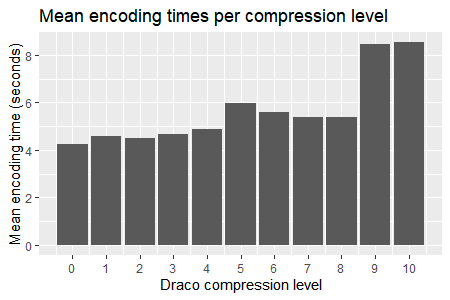
\includegraphics[scale=1]{figs/implementation/meanencodingtimes.png}
    \caption{Benchmark of mean encoding times per different Draco compression level}
    \label{fig:drcencodingtimes}
\end{figure}

Figure~\ref{fig:drcencodingtimes} shows that a higher compression level is not always slower than its predecessor.
This is counterintuitive, but the reason for it is likely that individual objects are being encoded, rather than one big mesh.
The different levels are probably determined based on their performance on larger meshes.
Small meshes are less complex and compression techniques will therefore behave differently on t.
Especially level 5 seems to be a bad choice if the encoding time is important, as it is even higher than 8 and 9.
It is not known why level 5 in specific performs badly, as it is not specified in the Draco specifications which techniques are used per level.

\begin{figure}[h!]
    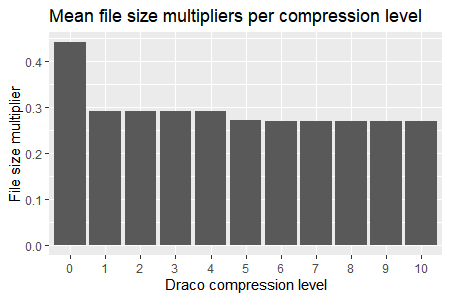
\includegraphics[scale=1]{figs/implementation/meanfilesize.png}
    \caption{Mean file size multipliers per Draco compression level}
    \label{fig:drcfilesizes}
\end{figure}

As for the file sizes, Figure~\ref{fig:drcfilesizes} shows the average file size multiplier of the Draco geometry compared to the original OBJ.
There are three groups: 0, 1 to 4, and 5 to 10.
Between the second two groups, the difference is probably because of the first one using the sequential connectivity method, and the second one using edgebreaker as this is said to be a main difference between compression levels.
Compression level 0 might compress the vertices only and not the connectivity.
Interestingly, despite level 5 taking relatively long to encode, its file size multiplier is not lower than several higher compression levels that encoded faster


\begin{figure}[h!]
    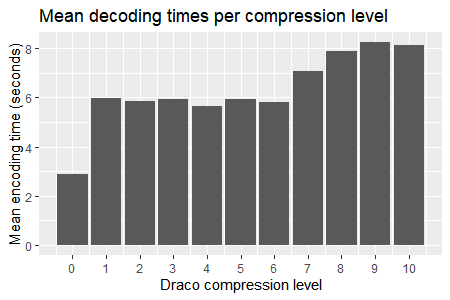
\includegraphics[scale=1]{figs/implementation/meandecodingtimes.png}
    \caption{Benchmark of mean decode times per different Draco compression level}
    \label{fig:drcdecodingtimes}
\end{figure}

Figure~\ref{fig:drcdecodingtimes} visualises the mean decoding times.
It is tested with the Draco C++ library however, as opposed to the decoder for JavaScript which might perform differently.
Between compression levels 1-6 there is not much of a difference, but 5 is again worse than 6.
Despite it being the middle option, it turns out to not be an optimal choice.
Level 0 is fast but it yields a relatively high file size.
Levels 7-10 take longer to decode than 6 despite resulting in similar file sizes.

Compression level 6 has just a slightly longer decoding time than 4, but it is smaller in size.
Concludingly, by having a low decoding time, small file size, and reasonable encoding time, it is the best option to use.






% The average OBJ size of all datasets converted to it is 49 MB. Misschien berekenen welke compressie het het meeste waard is? Bijvoorbeeld -> 49 MB wordt gecomprimeerd naar 20 MB. Het downloadt dan 6 seconden sneller. Maar ja decoding times lijken ook 6 seconden te zijn... Dus laat maar zitten denk ik




\section{Computer specifications}
The specifications of the used computer are listed in Table~\ref{tab:pcspecs} below as the time benchmark results are influenced by it.

\begin{table}[h!]
\begin{center}
 \begin{tabular}{ |c | c|} 
 \hline
Model & Lenovo Thinkpad P1 Gen 2 \\ 
\hline
\hline
CPU   & i7-9750H@2.6Ghz          \\
\hline
GPU   & Nvidia Quadro T1000      \\
\hline
OS    & Windows 10 Home 64-bits  \\ 
\hline
RAM   & 16 GB DDR4  \\          
\hline 
\end{tabular}
\caption{Specifications of computer used for benchmarking}
\label{tab:pcspecs}
\end{center}
\end{table}

